\subsection{UC17 - Visualizzazione elenco risultati ricerca prodotto}
\begin{figure}[H]
  \centering
  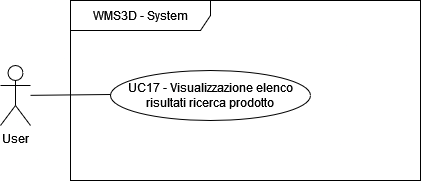
\includegraphics[width=0.8\textwidth]{UC_diagrams_11-20/UC17_sys.drawio.png}
   \caption{Diagramma UML UC17 - Visualizzazione elenco risultati ricerca prodotto}
\end{figure}
\begin{figure}[H]
  \centering
  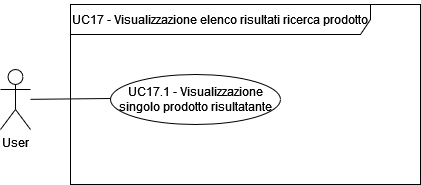
\includegraphics[width=0.8\textwidth]{UC_diagrams_11-20/UC17.drawio.png}
   \caption{Diagramma UML in dettaglio UC17 - Visualizzazione elenco risultati ricerca prodotto}
\end{figure}
\begin{itemize}
    \item \textbf{Attori:} User.
    \item \textbf{Pre-condizione:} L'utente ha ricercato un prodotto [UC16].
    \item \textbf{Post-condizione:} L'utente visualizza un elenco dei prodotti il cui nome corrisponde alla ricerca effettuata.
    \item \textbf{Scenario Principale:} L'utente, dopo aver ricercato un determinato nome, visualizza un elenco dei possibili prodotti corrispondenti alla ricerca, sempre se presenti. Se non ve ne dovesse essere nessuno, l'elenco sarà nullo.
    \item \textbf{Generalizzazioni:} -
    \item \textbf{Estensioni:} -
\end{itemize}


\subsection{UC17.1 - Visualizzazione singolo prodotto risultante}
\begin{itemize}
    \item \textbf{Attori:} User.
    \item \textbf{Pre-condizione:} L'utente ha ricercato un prodotto [UC16] e sta visualizzando l'elenco dei risultati corrispondenti [UC17]. Almeno un prodotto deve essere stato creato [UC13].
    \item \textbf{Post-condizione:} Il prodotto risultante dalla ricerca viene selezionato [UC15].
    \item \textbf{Scenario Principale:} Per ogni singolo prodotto risultante dalla ricerca, l'utente ne visualizza il nome e questo viene selezionato sulla libreria e, se posizionato, sul render 3D.
    \item \textbf{Generalizzazioni:} -
    \item \textbf{Estensioni:} -
\end{itemize}